\section{Part~I: The Spectral Barrier}\label{sec:part1}

The fundamental capacity of a physics-informed neural network to capture the dynamics of a PDE heavily depends on its ability to resolve the necessary range of spatial and temporal frequencies. When addressing advection-dominated flows, networks frequently exhibit an inability to converge, a phenomenon often attributed to spectral bias. In this section, we systematically investigate the onset of this barrier, the efficacy of standard mitigation techniques, and the underlying conditioning of the optimization landscape that drives this pathology.

\subsection{Experiment 1: Spectral Bias Phase Transition}\label{sec:exp1}

To quantify the exact boundary at which standard \PINN{} architectures fail to resolve advective physics, we systematically evaluate the 1D linear advection equation across an escalating sequence of advection coefficients, $\betaAdv \in \{1, 5, 10, 30, 50, 100\}$. The network's predictive performance demonstrates a stark and sudden phase transition from successful convergence to total structural failure. At low advection velocities ($\betaAdv = 1$ and $\betaAdv = 5$), the relative $\Ltwo$ errors remain negligible at $0.0047$ and $0.0058$, respectively, indicating that the network easily resolves the underlying wave dynamics. As the advection coefficient increases to $\betaAdv = 10$, the error rises moderately to $0.0414$, showing early signs of optimization strain. However, a critical failure threshold is consistently observed at $\betaAdv = 30$, where the $\Ltwo$ error abruptly jumps to $0.9079$. Further increases to highly stiff regimes at $\betaAdv = 50$ and $\betaAdv = 100$ yield catastrophic relative $\Ltwo$ errors of $0.9630$ and $0.9923$, respectively. These elevated error metrics reveal complete structural failure of the network to approximate the target function, reducing the prediction to non-physical mean states.

\begin{figure}[htpb]
    \centering
    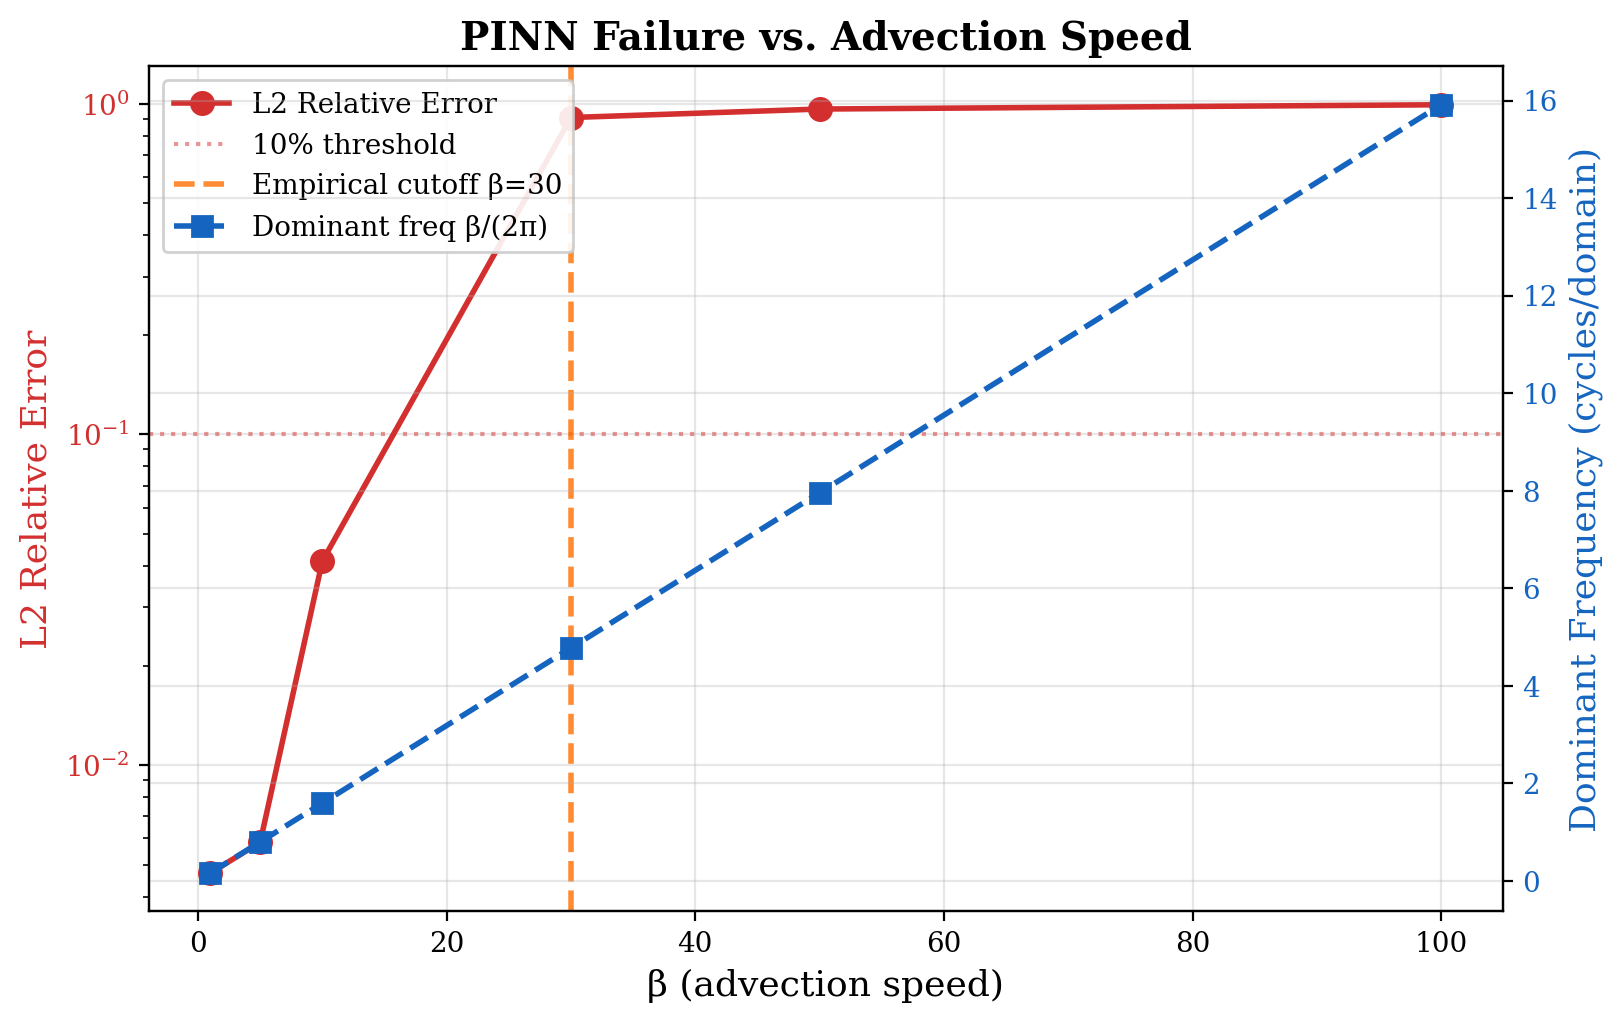
\includegraphics[width=\linewidth]{results/exp1/l2_vs_beta.png}
    \caption{Relative $\Ltwo$ error as a function of advection speed $\betaAdv$ for the standard \PINN{} (4 hidden layers, 64 neurons, \texttt{tanh} activation). A sharp phase transition is visible near $\betaAdv = 30$, above which the $\Ltwo$ error exceeds 0.88 across all tested configurations. The dashed horizontal line marks the failure threshold ($\Ltwo = 0.10$).}
    \label{fig:exp1_l2_vs_beta}
\end{figure}

The mechanism driving this abrupt transition is highly consistent with the spectral bias inherent to continuous neural networks \cite{Rahaman2019spectral}. Standard multi-layer perceptrons inherently prioritize fitting low-frequency, smooth components of the target function during the initial phases of gradient descent. As the advection coefficient $\betaAdv$ increases, the PDE's characteristic curves steepen, requiring the network to resolve proportionally higher spatial and temporal frequencies to accurately advect the initial conditions across the domain. Spectral analysis of the residual error field reveals a sharp empirical cutoff frequency of $f_c = 4.7746$ explicitly at the critical $\betaAdv=30$ threshold. Beyond this specific frequency limit, the predicted power spectrum rapidly decays and merges with the numerical noise floor, rendering the network effectively blind to the fine-scale dynamics required by the underlying physical system. This specific spectral truncation suggests that the empirical failure is deeply tied to the network's fundamentally bounded frequency resolution capabilities.

\subsection{Experiment 2: Activation Function Mitigation}\label{sec:exp2}

A common strategy proposed in the literature to circumvent spectral bias involves replacing the standard $\tanh$ activation with alternatives possessing higher non-zero derivatives, or by explicitly introducing high-frequency components into the input coordinates via random Fourier features. To rigorously test the viability of these mitigations, we evaluate seven distinct activation configurations at the established critical failure threshold of $\betaAdv=30$: the standard $\tanh$, $\sin$ (representing SIREN-like architectures), $\text{swish}$, $\text{gelu}$, and random Fourier features with logarithmically increasing scale factors ($\sigma \in \{1, 10, 100\}$).

\begin{figure}[htpb]
    \centering
    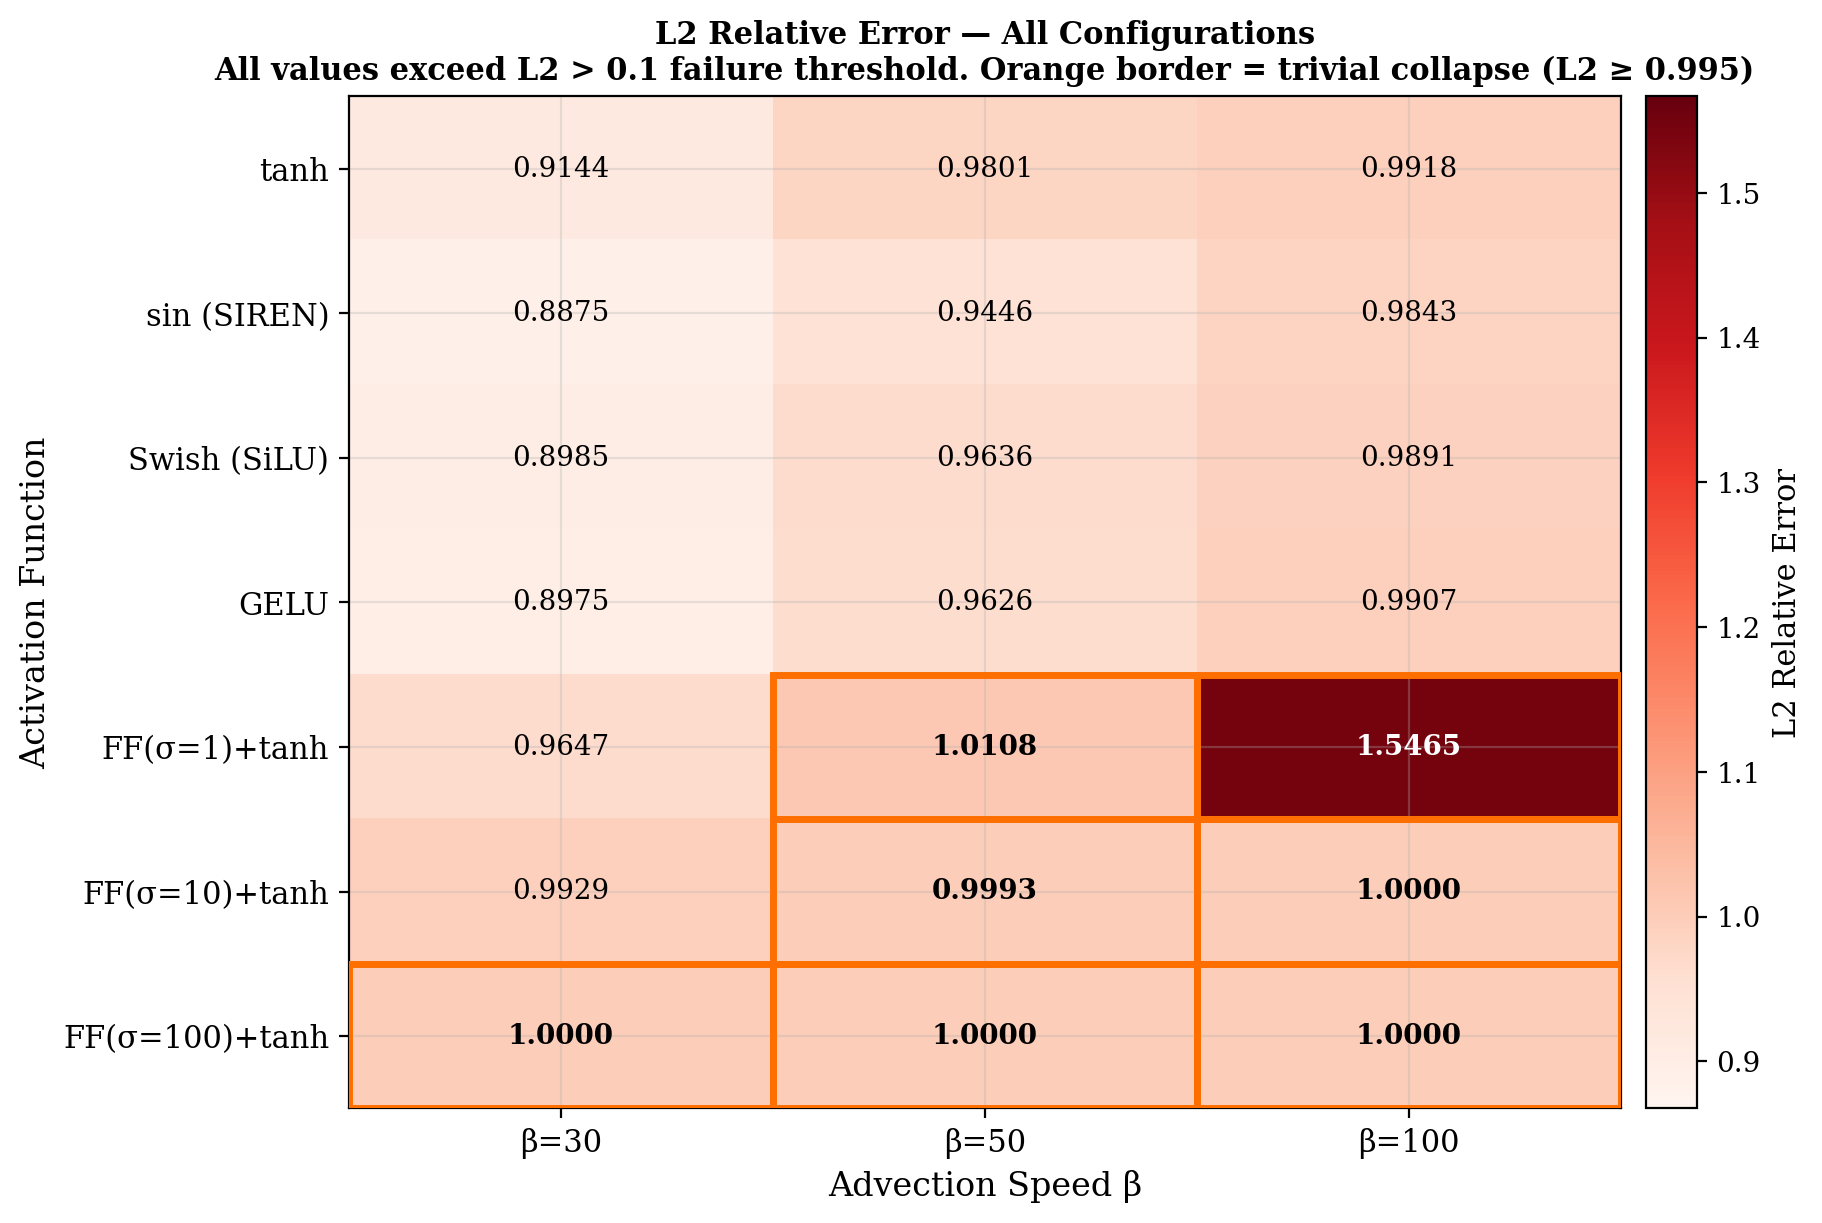
\includegraphics[width=\linewidth]{results/exp2/l2_heatmap.png}
    \caption{Relative $\Ltwo$ errors across various activation functions and Fourier feature scales evaluated at $\betaAdv=30$. None of the tested activation configurations successfully mitigate the spectral failure, demonstrating robustness of the barrier against local non-linear substitutions.}
    \label{fig:exp2_activation_comparison}
\end{figure}

The experimental results demonstrate that the spectral barrier is remarkably robust against activation substitution. At the $\betaAdv=30$ threshold, the baseline $\tanh$ architecture yields an $\Ltwo$ error of $0.9144$\,\footnote{The tanh baseline at $\betaAdv=30$ differs slightly between Experiments~1 and~2 (0.9079 vs.\ 0.9144) due to differing random seeds; both experiments use 10,000 collocation points. Both values are consistent with the observed run-to-run variance at this $\betaAdv$ level, confirming the discrepancy is attributable to training stochasticity rather than a configuration error.}. The alternative standard activations perform similarly poorly; the $\text{swish}$ activation yields $0.8985$, the $\text{gelu}$ activation yields $0.8975$, and the periodic $\sin$ activation provides the lowest, yet still catastrophic, error of $0.8875$. Attempts to force high-frequency resolution via random Fourier features similarly fail to pierce the spectral barrier; the lightly scaled $\sigma=1$ configuration yields an error of $0.9647$, and the $\sigma=10$ configuration produces an error of $0.9929$. Notably, the highly oscillatory $\sigma=100$ Fourier feature configuration exhibits a condition termed Trivial Collapse, resulting in a maximal $\Ltwo$ error of $1.0000$. This specific error bound indicates that the network converges precisely to the zero-function attractor, trapped in a pathologically flat region of the highly non-convex PDE gradient landscape. Explicitly, across all structural configurations tested, no single activation function successfully pierces an $\Ltwo$ error of $0.8875$ at $\betaAdv=30$. This persistent failure regime suggests that simply modifying the local, non-linear basis of the network is entirely insufficient to overcome the global conditioning bottlenecks induced by stiff advection.

\subsection{Experiment 3: NTK Condition Number Analysis}\label{sec:exp3}

To determine whether the empirically observed spectral failure is a dynamic byproduct of the gradient descent training process or a fundamental geometric constraint inherent to the architecture, we analyze the conditioning of the empirical Neural Tangent Kernel (NTK). Crucially, this NTK profiling is performed exactly at initialization—before any training steps occur. We systematically profile $25$ distinct multi-layer perceptron architectures, spanning widths from $16$ to $256$ neurons and depths from $2$ to $8$ hidden layers, all evaluated at the severe advection regime of $\betaAdv=50$.

\begin{figure}[htpb]
    \centering
    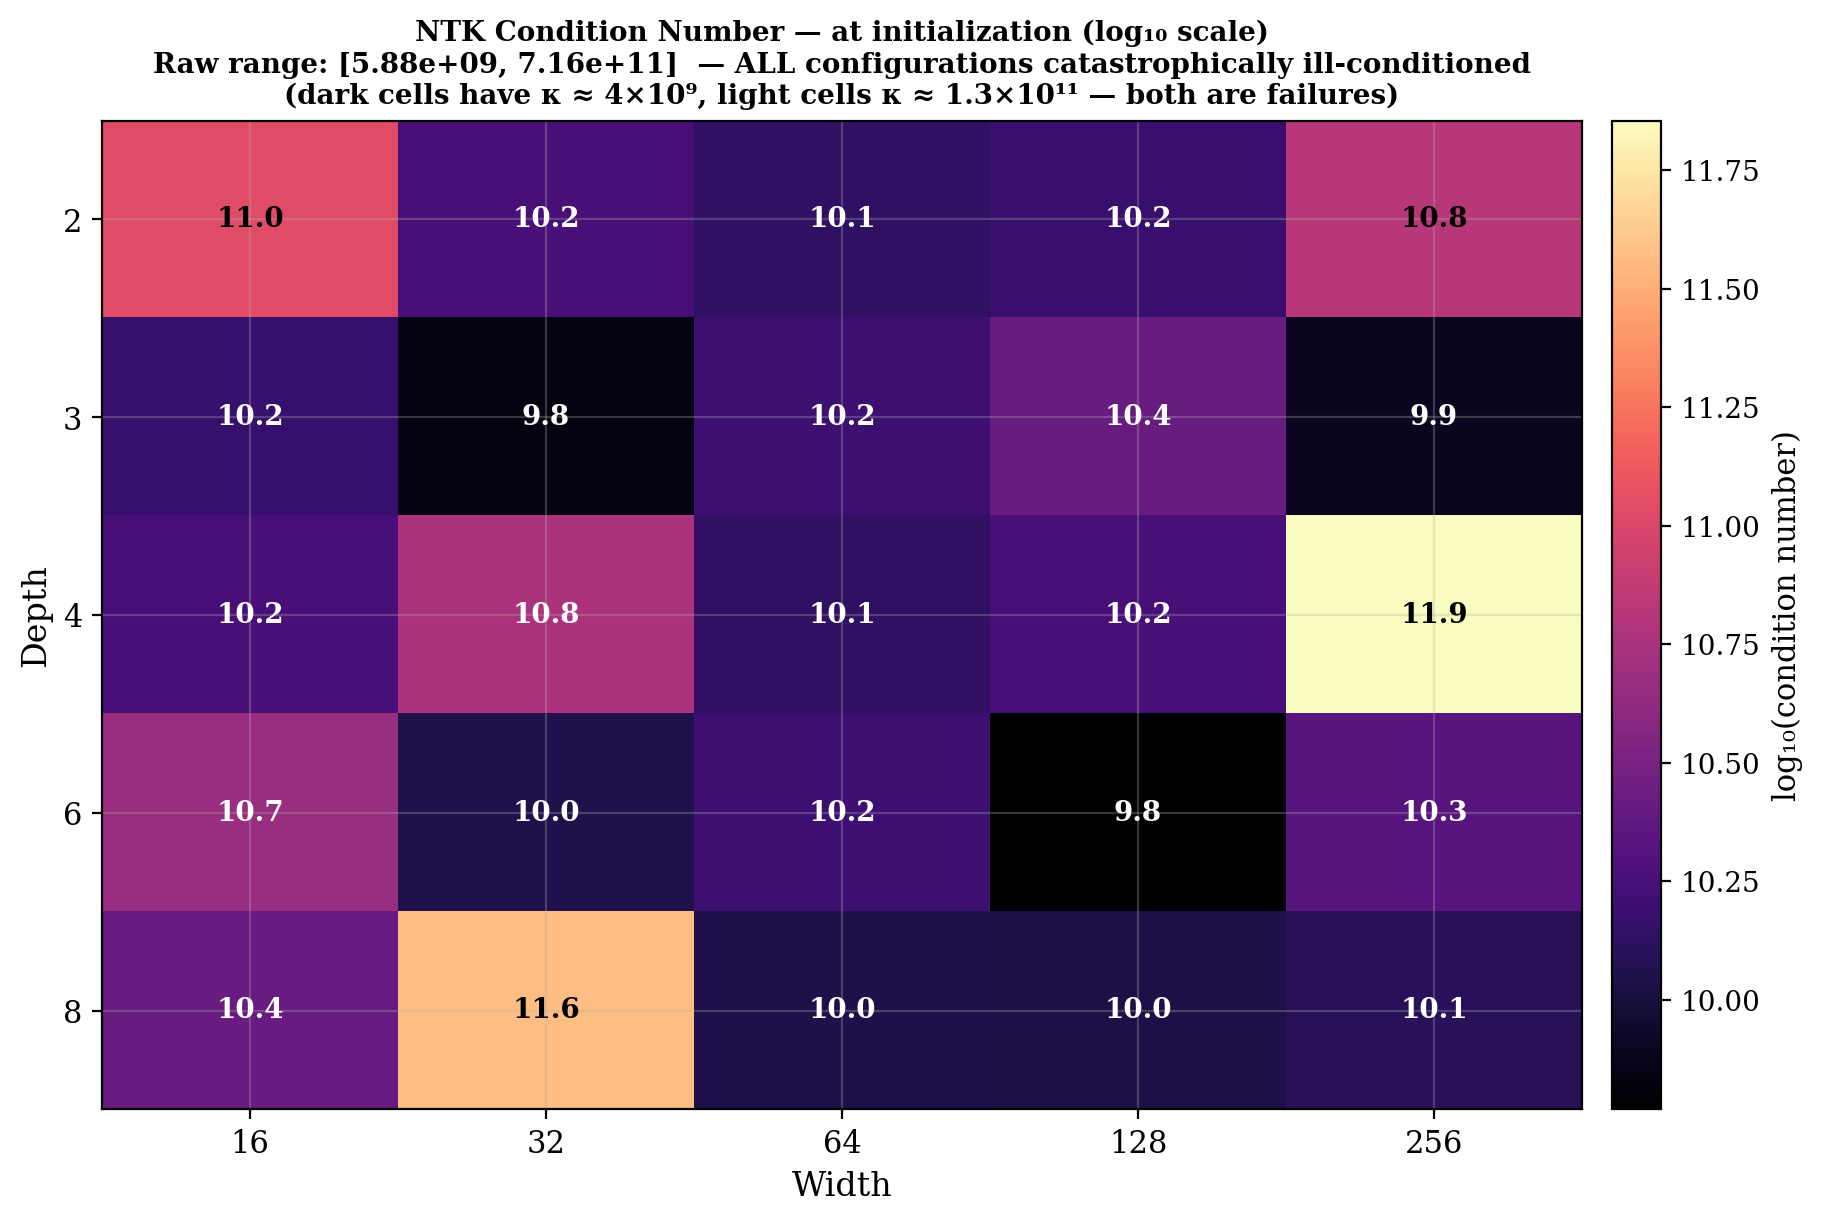
\includegraphics[width=\linewidth]{results/exp3/ntk_eigenvalue_heatmap.png}
    \caption{Heatmap of NTK condition numbers at initialization across 25 architectures (varying depth and width) at $\betaAdv=50$. All architectures demonstrate severe, catastrophic ill-conditioning regardless of capacity scaling.}
    \label{fig:exp3_ntk_heatmap}
\end{figure}

The eigenvalue analysis reveals catastrophic ill-conditioning across the entire, expansive architectural sweep. The NTK condition numbers, denoted as $\kNTK$, range from an enormous minimum of $5.8774 \times 10^{9}$ up to a staggering maximum of $7.1558 \times 10^{11}$. Correspondingly, the eigenvalue power-law decay exponents, $\alpha$, fall within the strict range of $2.8359$ to $3.3840$. This steep decay rate indicates that the kernel's spectrum drops precipitously across the frequency domain, leaving high-frequency eigen-directions with effectively zero support during gradient flow. Consequently, the final test performance remains universally poor across all scales; the relative $\Ltwo$ errors across all 25 evaluated architectures vary tightly between $0.9685$ and $1.1266$, demonstrating total failure irrespective of the network's raw parameter count. The ill-conditioning pre-exists training, appearing at initialization, suggesting the failure is embedded in the representational geometry rather than learned.

\subsection{Synthesis: Structural Nature of the Spectral Barrier}

The empirical evidence compiled from these three targeted experiments paints a cohesive and challenging picture of \PINN{} failure in advection-dominated regimes. The precise phase transition marking the onset of spectral failure is clearly and independently measurable from two distinct perspectives: dynamically, as evidenced by the terminal spectral error analysis and the $f_c = 4.7746$ frequency cutoff measured after training in Experiment 1; and statically, long before training even commences, as demonstrated by the catastrophic NTK condition numbers spanning $10^{9}$ to $10^{11}$ evaluated strictly at initialization in Experiment 3. Both perspectives independently agree: the continuous optimization landscape is structurally hostile to the simultaneous resolution of the multi-scale physical features implicitly required by stiff PDEs.

Furthermore, the extreme robustness of this spectral barrier against standard architectural interventions underscores its fundamental, systemic nature. As demonstrated in Experiments 2 and 3, neither the strategic selection of specialized activation functions nor the brute-force capacity scaling through substantially wider and deeper networks resolves the underlying pathology. Instead of being a superficial training anomaly that can be tuned away with hyperparameter sweeps, the spectral barrier manifests as a strict, invariant representational constraint. Attempts to bypass this constraint—such as injecting high-frequency components via highly scaled Fourier features—merely trade one manifestation of failure for another, directly resulting in the trivial zero-function collapse. This intertwined pathology indicates a much deeper, systemic issue governing the loss manifold; effectively addressing the spectral barrier intrinsically requires examining how these harsh geometric constraints drive destructive interference during optimization. This intricate connection between spectral bias and competing loss terms is explored in detail through the lens of gradient pathology in Part II. One limitation of the NTK analysis presented here is its restriction to the network's state at initialization; while empirical evidence suggests these initial conditioning bottlenecks strongly predict final failure, the evolution of the NTK during training across diverse architectures remains an open area for future investigation.
